\section{Machine learning approach}\label{sec:machine_learning}
\begin{figure*}[ht]
\begin{minipage}{0.62\textwidth}
\begin{tabular}{|c|c|c|c|}\hline
    Model &Training data&Test data&Error  \\\hline
    \makecell{
\includegraphics[scale=0.5]{visualisation/blue_square.png}\\original}&swimmer info, 50m&swimmer info, 50m&7.97\\\hline
    
\includegraphics[scale=0.5]{visualisation/yellow_circle.png}&\makecell{swimmer info, 50m,\\ true 100m}& \makecell{swimmer info, 50m,\\ true 100m}&5.77\\\hline
    
\includegraphics[scale=0.5]{visualisation/red_circle.png}&\makecell{swimmer info, 50m,\\ true 100m}&\makecell{swimmer info, 50m,\\ predicted 100m}&8.30\\\hline
    
\includegraphics[scale=0.5]{visualisation/green_triangle.png}&\makecell{swimmer info, 50m,\\ predicted 100m}&\makecell{swimmer info, 50m,\\ predicted 100m}&7.67\\\hline
\end{tabular}
\end{minipage}
\begin{minipage}{0.38\textwidth}
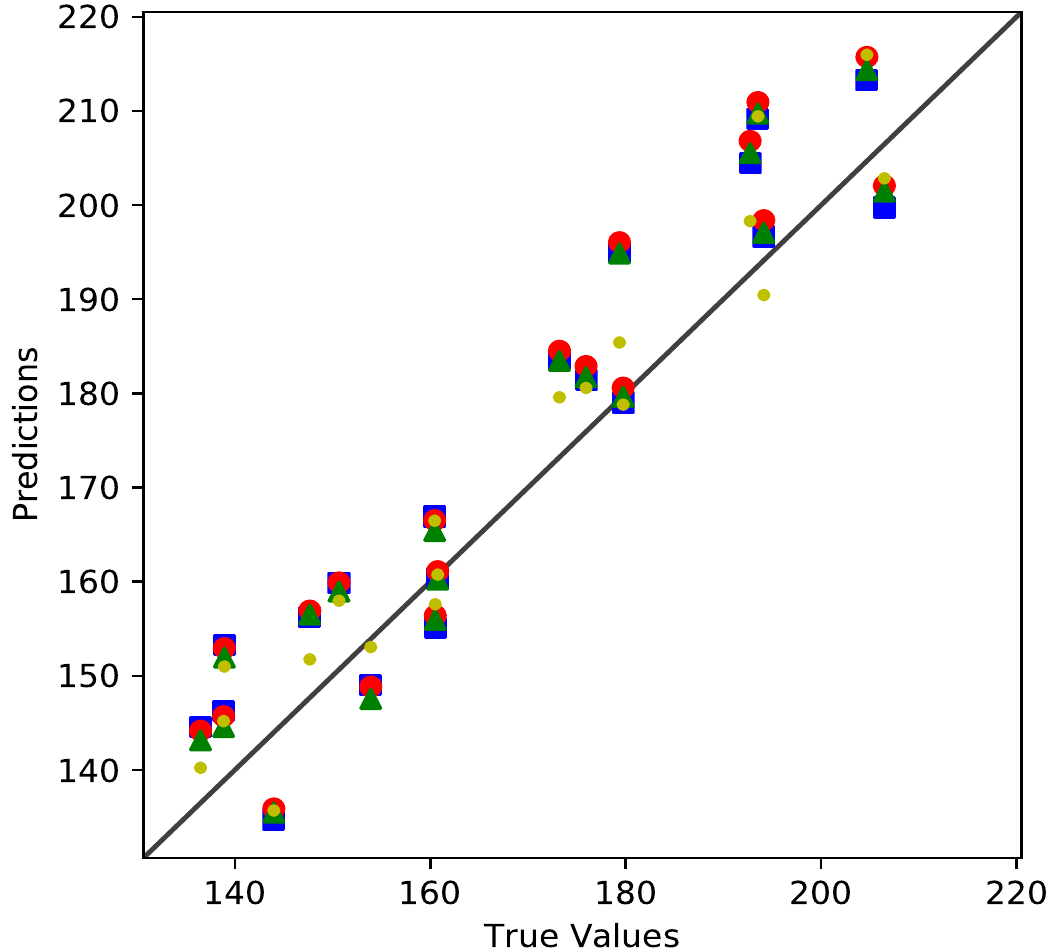
\includegraphics[width=\textwidth]{visualisation/eval_200m_variations.png}
\end{minipage}
\caption{Comparison of different 200m approaches}
\label{fig:200m_variations}
\end{figure*}
Using these datasets, we train machine learning models to predict the longer distance times. We use Tensorflow\footnote{\url{https://www.tensorflow.org/} accessed 03.01.2020} for training our machine learning models. Tensorflow offers a well-documented and flexible ecosystem as well a the tensorflow-lite package that makes it possible to use trained models on mobile devices.\\
\subsection{Model selection}
We will train two separate models, one for the 100m and one for the 200m prediction. Our models must return continuous output values; thus, we need to solve a regression instead of a classification task. Therefore, we use the regression model explained in the Tensorflow tutorials \footnote{\url{https://www.tensorflow.org/tutorials/keras/regression}, accessed 02.01.2020}. As we have seen in the previous section, our data is linearly separable thus our model does not need a hidden layer to fit the data.
For the training itself, we randomly split our training data into a training and validation subset with a fraction of $\frac{1}{3}$ and use the validation set to evaluate the current model. As our output must be continuous, we can only use activation functions that do not saturate, e.g. linear function or ReLU. The linear function can return negative values, while ReLU can only return values greater or equal to zero. As the predicted times are greater than zero, it makes no difference which of these activation functions we use. Besides, as per common knowledge \cite{Reed.1999}, we use mean-squared error as loss function.\\
We evaluate the final models with a separate test dataset and mean absolute error as metric.\\
\begin{figure}[ht]
\begin{centering}
\begin{tabular}{|cc|c|c|c|}\hline
    &&\multicolumn{3}{c|}{\textbf{Units}}\\
    & & 16 & 32 & 64 \\\hline
    \multirow{2}{*}{\textbf{rmsprop}}&100m&1.94&1.90&1.97\\\cline{2-5}
    &200m&5.35&5.49&5.92\\\hline
    \multirow{2}{*}{\textbf{adam}}&100m&4.88&5.28&2.48\\\cline{2-5}
    &200m&10.40&8.55&8.47\\\hline
\end{tabular}
\captionof{table}{Mean absolute error for different units in input layer}
\label{tab:hyperparam_units}
\end{centering}
\end{figure}
In order to find the best model, we vary two parameters: The number of neurons in the Dense input layer and the optimiser used to fit our data. Therefore, we train models using $\{16, 32, 64\}$ neurons and try different optimisers offered by the keras library\footnote{\url{https://keras.io/optimizers/}, accessed 03.01.2020}, i.e. Adam or RMSprop. For both optimisers, we use their default learning rates of $0.001$ The models are trained using the training data and tested against the validation data. The results are presented in Table \ref{tab:hyperparam_units}.\\
We can see that RMSprop is the best optimiser; thus, we use RMSprop with 32 units for the 100m prediction and RMSprop with 16 units for the 200m prediction. We train the model in 500 epochs and spltting the data into a batch size of 32.
\subsection{Model evaluation}
We evaluate the resulting models using the test dataset. Figure \ref{fig:eval_model} shows the scatter of the predicted and the correct 100m times as well as the predicted and correct 200m times. The black line in each plot represents the optimum, where predicted and correct times are identical thus the closer the dots are to this line, the better is the model.
\begin{figure}[ht]
    \begin{minipage}{0.23\textwidth}
    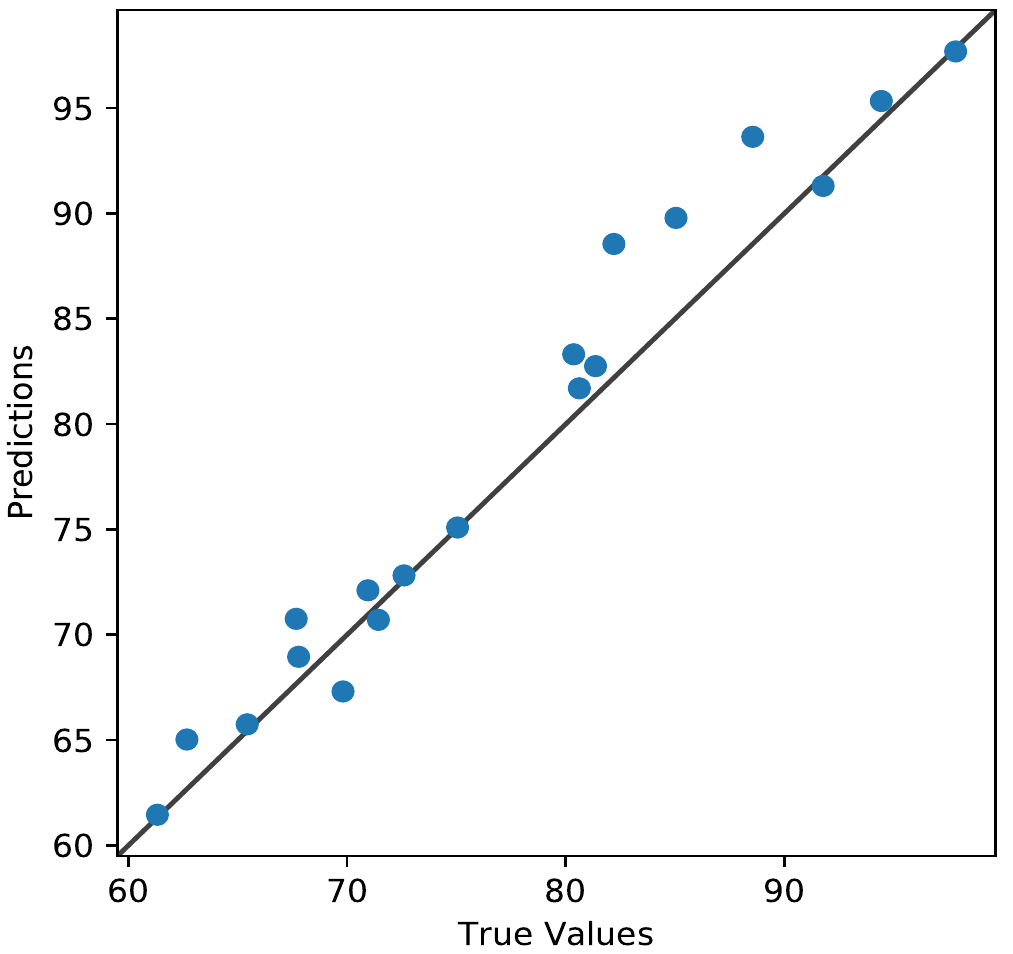
\includegraphics[width=\textwidth]{visualisation/eval_100m.png}
\end{minipage}
\begin{minipage}{0.23\textwidth}
    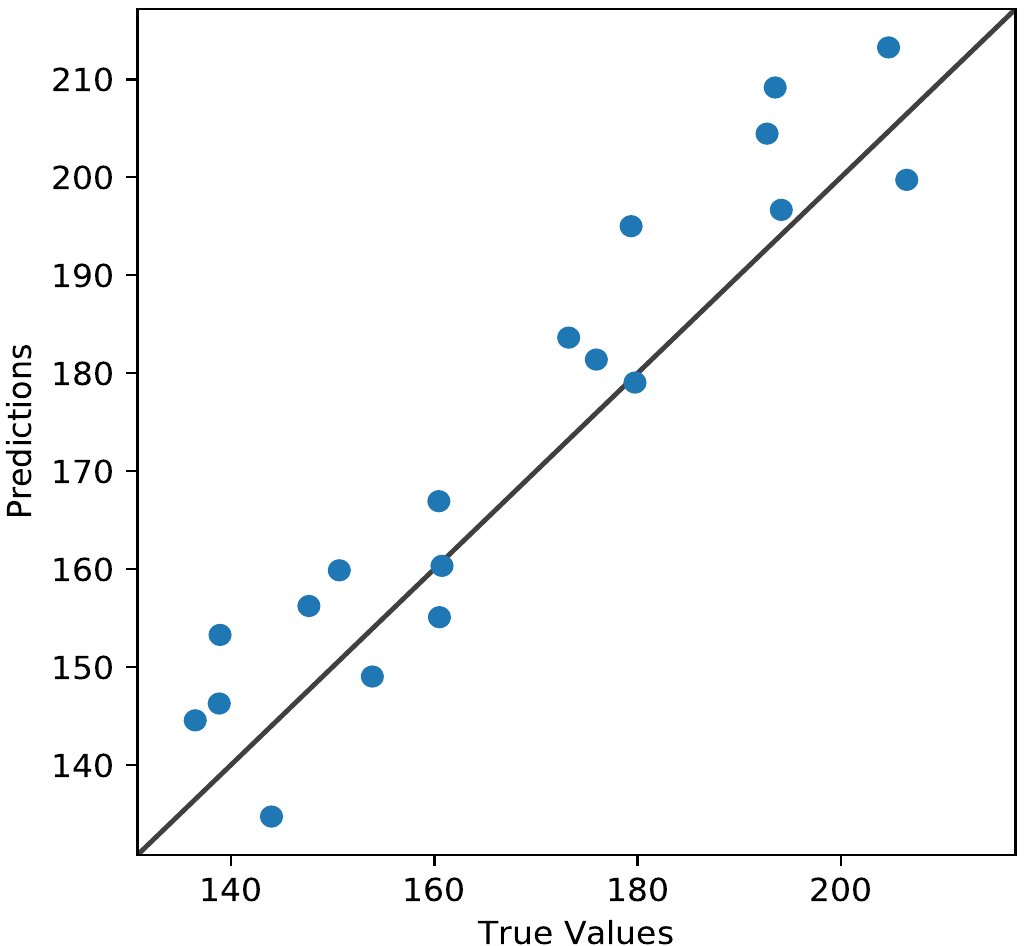
\includegraphics[width=\textwidth]{visualisation/eval_200m.png}
\end{minipage}
\caption{Evaluation of 100m (left) and 200m (right) model}
\label{fig:eval_model}
\end{figure}
The models achieve a mean-absolute error of $1.83$ for the 100m model and $7.97$ for the 200m model. We consider the 100m prediction as successful thus we use this model in our application.\\
The 200m prediction, however, has deficits. A potential improvement could be to include the 100m times in the 200m prediction. In order to evaluate this idea, we train two additional models. For the first model, we add the correct 100m times to the training data and for the second model, we use the 100m model to predict the 100m times and add these times to the training data. Figure \ref{fig:200m_variations} evaluates the four resulting models. The small yellow circles use the correct 100m times for training and prediction. It is important to mention that this model is only for theoretical analysis and does not apply to our real-world problem as we do not know the correct 100m times when we predict new samples. However, this model shows that using the 100m times for the 200m prediction can indeed improve the results. The models using the predicted 100m times for the 200m prediction do not perform better than the original model. Moreover, we can see in the plot that these models almost ignore the 100m time as their predicted times are nearly identical. A reason for this is that the 100m prediction model is not good enough to be helpful for the 200m prediction. Finally, using the 100m times for the 200m model is a good idea but does not work in practice; thus, we use the original 200m model in our application.